\documentclass{beamer}

\mode<presentation>
{
  \useoutertheme{default}
}

\beamertemplatenavigationsymbolsempty
\setbeamertemplate{frametitle}[default][center]

\title{Mathematical models of invasion and evolution in adenocarcinomas}
\author{Chay Paterson}
\institute{University of Washington}
\date[\today]{}

\begin{document}

\frame{\titlepage}

\begin{frame}
\frametitle{What is cancer?}
% List of hallmarks, emphasise two

% diagram from hallmarks paper

\begin{center}
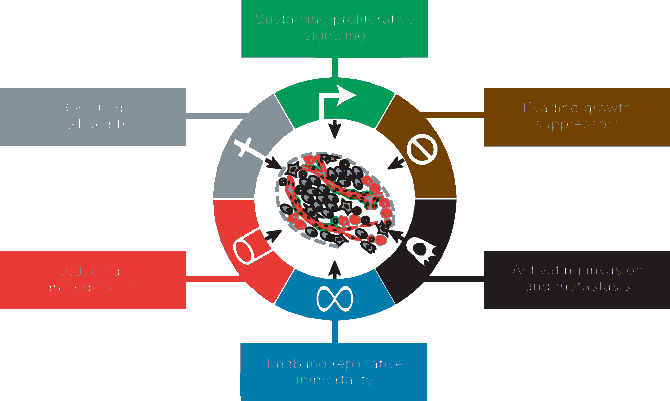
\includegraphics[width=1.0\textwidth]{images/hallmarks2011.pdf}
\end{center}

\hrule
\;

\tiny{D. Hanahan, and R. A. Weinberg. ``The hallmarks of cancer: The Next Generation.'' \emph{Cell}
144.5 (2011): 646-674}
\end{frame}

\begin{frame}
\frametitle{\emph{In vitro} experiments}
% J.P. Landry's experiments
\begin{columns}[c]
    \column{0.4\textwidth}
    \begin{enumerate}
        \item Lesions are spheroidal
        \item Expanded with steady speed $0.03\; \mathrm{mm}/\mathrm{hr}$
        \item Shed cells at rate $\propto 0.05\;\mathrm{hr}^{-1}
        \mathrm{mm}^{-2} \times $ surface area
    \end{enumerate}
    
    \column{0.6\textwidth}
    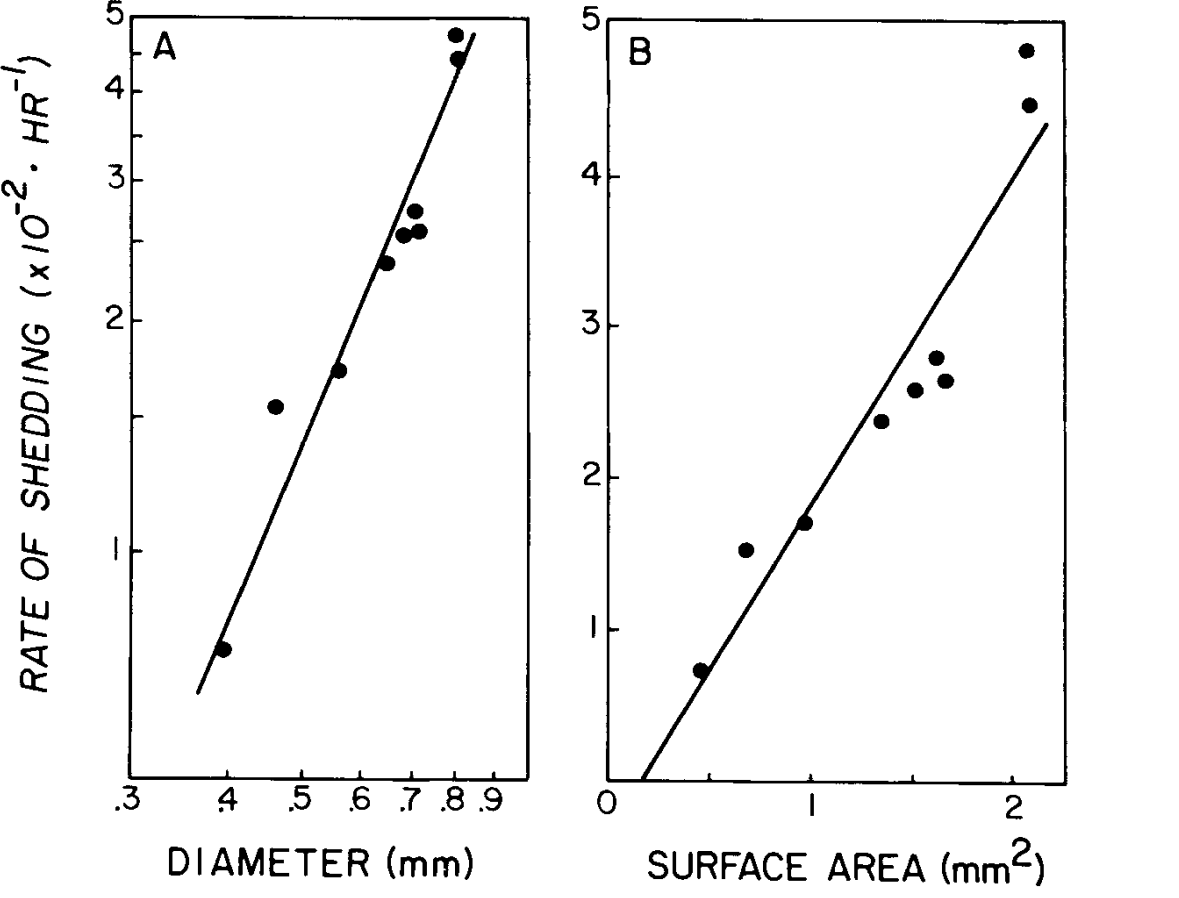
\includegraphics[width=1\linewidth]{images/JLandry_JCellPhys_1981_small.png}
\end{columns}

 \;
 \hrule
 \;
\tiny{J. Landry \emph{et al.}, ``Shedding of mitotic cells from the surface of multicell spheroids
during growth'', \emph{Journal of cellular physiology} 106.1 (1981): 23-32}
\end{frame}

\begin{frame}
\frametitle{\emph{In vivo} experiments}
%K. Iwata's experiments

\begin{center}
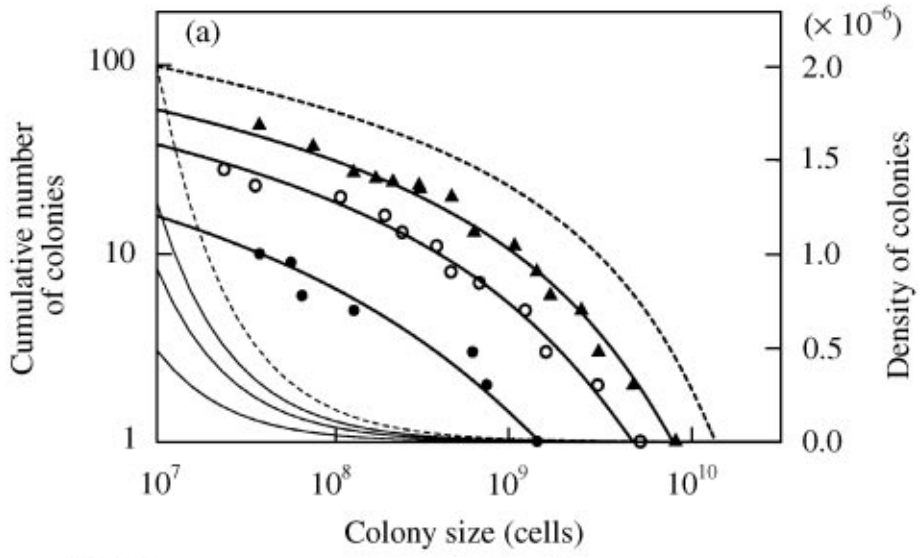
\includegraphics[width=0.75\textwidth]{images/KIwata_2000_Large.png}
\;

\small{Explains entire size distribution \emph{and} growth rate with \emph{two
equations}!}
\end{center}
\;
\hrule
\;

\tiny{K. Iwata, K. Kawasaki, and N. Shigesada, ``A dynamical model for the growth
and size distribution of multiple metastatic tumors.'' \emph{Journal of theoretical
biology} 203.2 (2000): 177-186}
\end{frame}

\begin{frame}
    \frametitle{Evolutionary dynamics}
    Initially, assume a completely linear space of possible genotypes:
    % o--o--o
    \begin{center}
    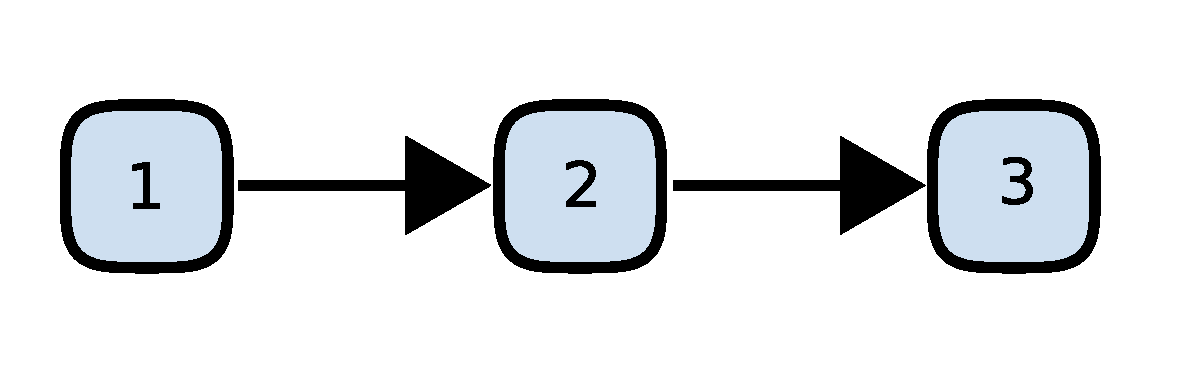
\includegraphics[width=0.8\textwidth]{images/linearlandscape.pdf}
    \end{center}
\end{frame}


\begin{frame}
\frametitle{Lattice simulations}

\begin{columns}[c]
    \column{0.5\textwidth}
    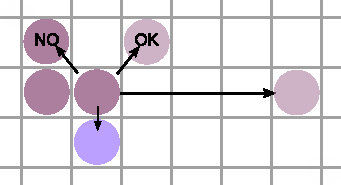
\includegraphics[width=1\textwidth]{images/latticemodel.pdf}
    \;

    Controlled by:
    \begin{itemize}
        \item Birth/death rates $b_n$, $d_n$
        \item Migration probability $M$
        \item Mutation probability $p_\mu$
    \end{itemize}
    \column{0.5\textwidth}
    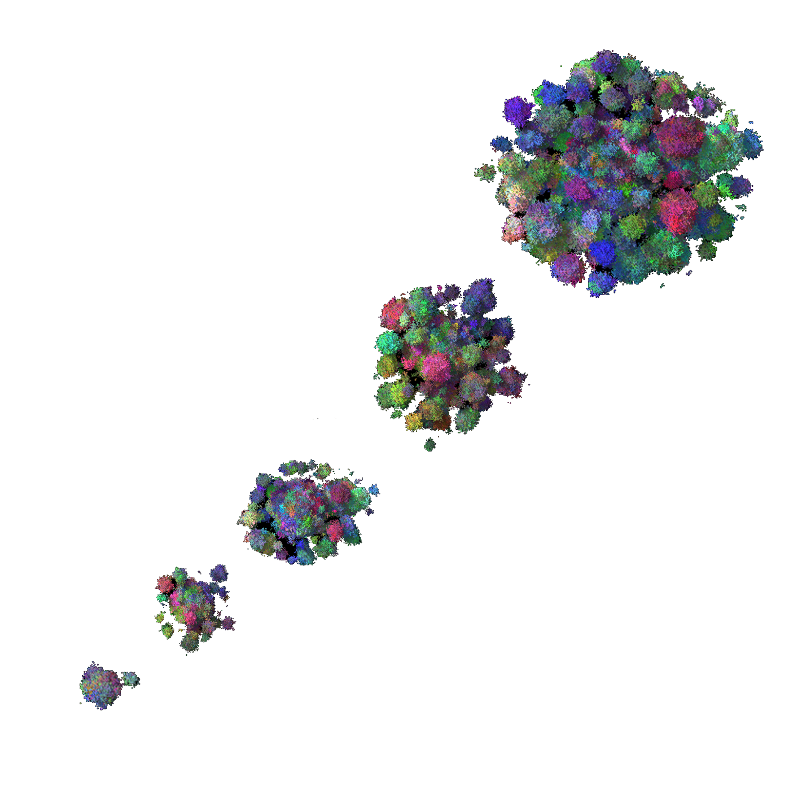
\includegraphics[width=1\linewidth]{images/GraphBG-2.png}
\end{columns}
\end{frame}

\begin{frame}
\frametitle{Lattice simulations}
\begin{columns}[c]
    \column{0.5\textwidth}
    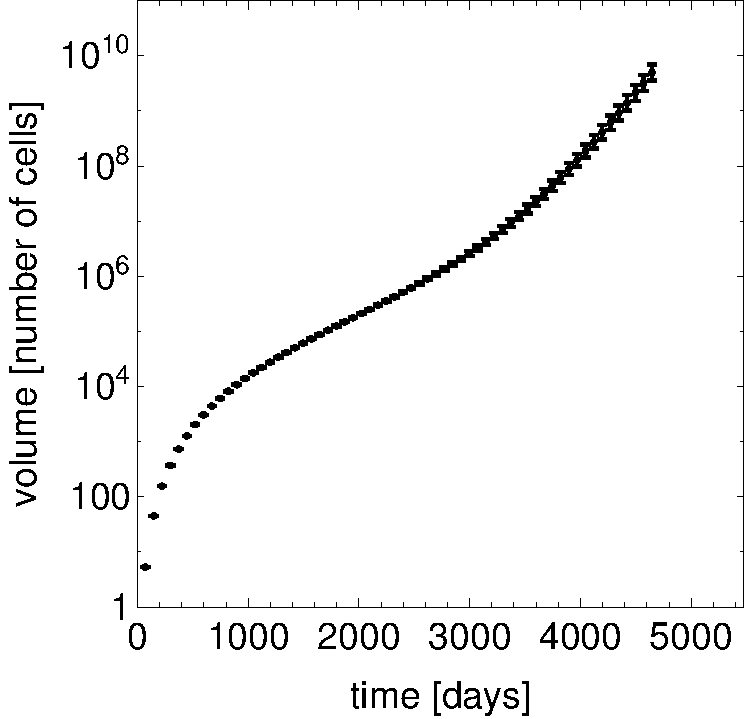
\includegraphics[width=1\textwidth]{images/SimpleModel1.pdf} 
    \column{0.5\textwidth}
    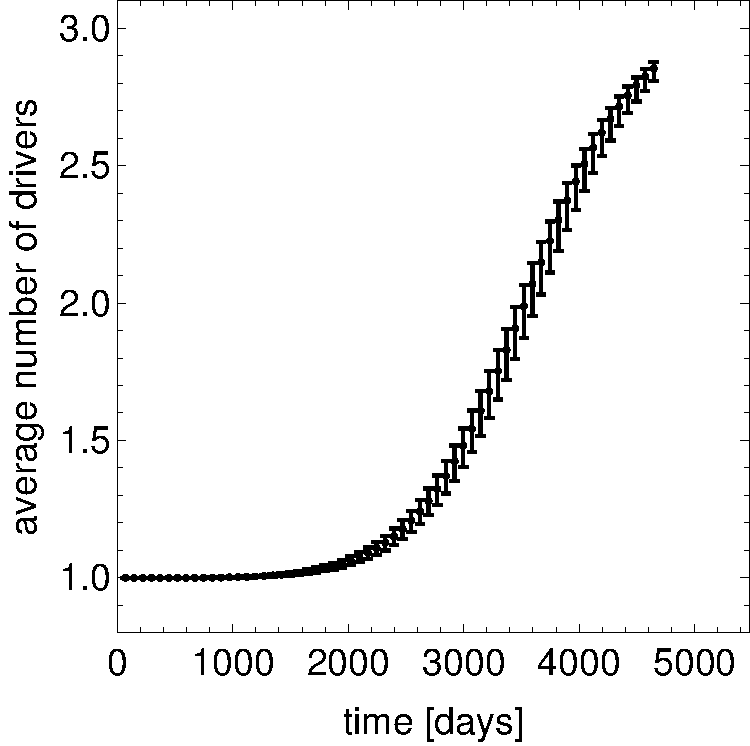
\includegraphics[width=1\textwidth]{images/SimpleModel2.pdf} 
\end{columns}
\end{frame}

% TODO diagram for analytical model

\begin{frame}
    \frametitle{Analytical model}

\begin{center}
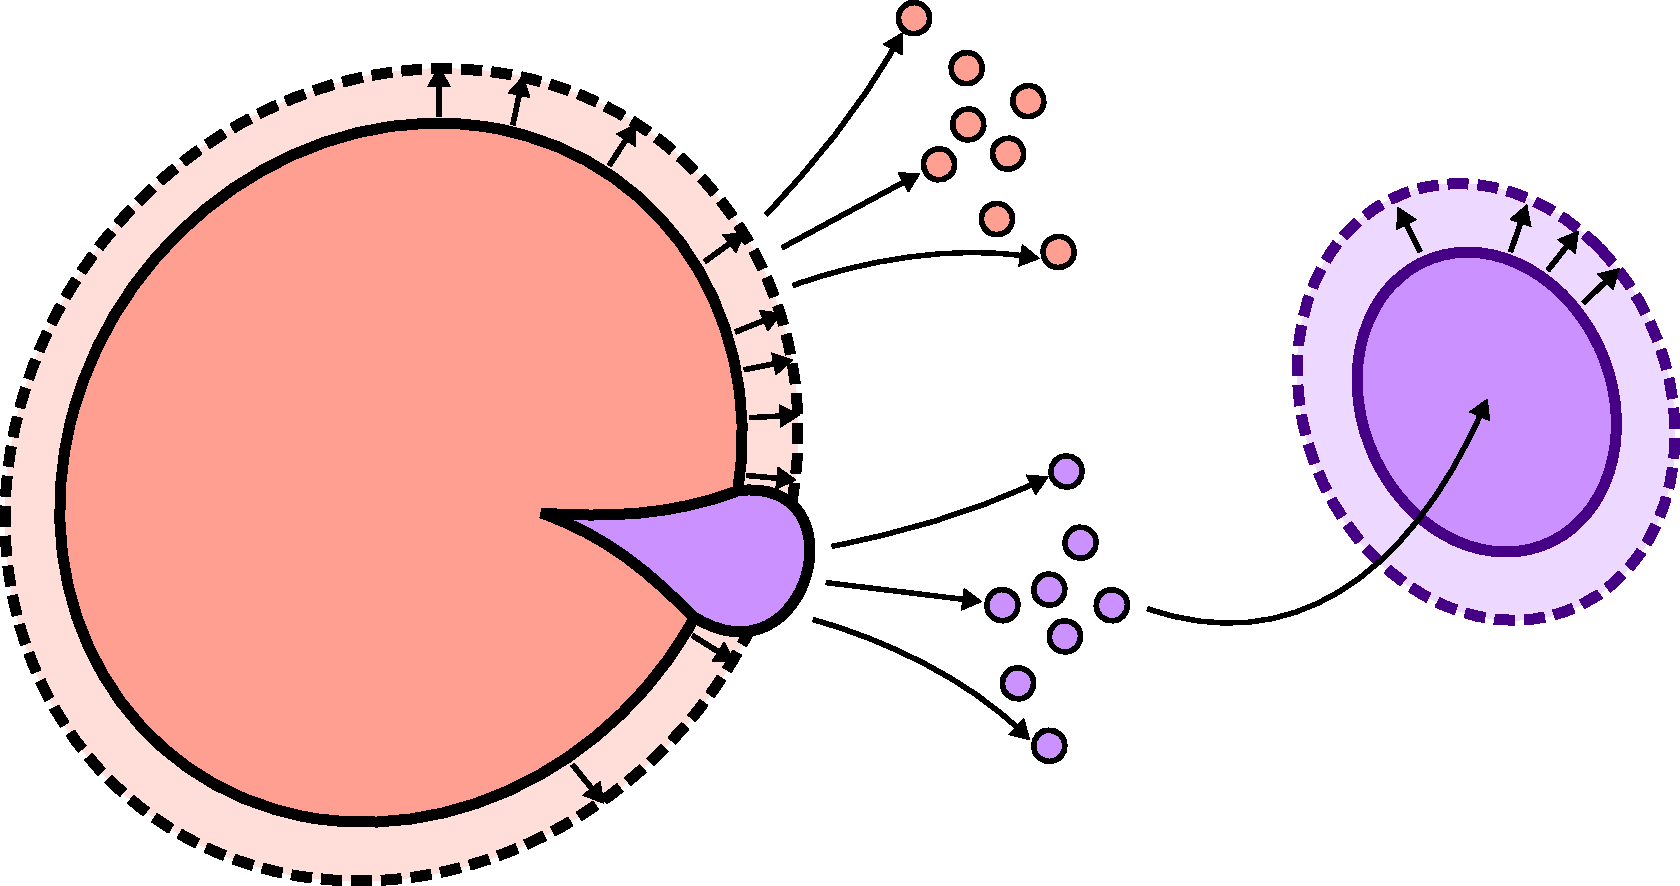
\includegraphics[width=1.0\textwidth]{images/OldModel.pdf}
\end{center}

\end{frame}

\begin{frame}
\frametitle{Analytical model}

Two equations:
\begin{enumerate}
    \item growth
    \item invasion+mutation
\end{enumerate}
\begin{align}
    \partial_t f_n(a,t) &+ \partial_a f_n(a,t) = 0\\
    f_n(0,t) &= \int_0^\infty r_n(a)\phi_n(a)f_n(a,t) da \nonumber \\
    &\; + \int_0^\infty
    (1-r_{n-1}(a))\phi_{n-1}(a) f_{n-1}(a,t) da
\end{align}

\;
\hrule
\;

\begin{center}
\tiny{Chay Paterson, Martin A. Nowak, Bartlomiej Waclaw, ``An exactly
solvable, spatial model of mutation accumulation in cancer'', \emph{Scientific
Reports} 2016}
\end{center}
\end{frame}

\begin{frame}
\frametitle{Exact solution!}
    \begin{enumerate}
        \item Total number and total mass of lesions of sub-type $n$ grows
        exponentially with growth rate $G_n$ satisfying
    \end{enumerate}

    \begin{equation*}
        \int_0^\infty \phi_n(a) \mathrm{e}^{-G_n a} da = 1
    \end{equation*}

    \begin{enumerate}
        \setcounter{enumi}{1}
        \item E.G. for $\phi_n = 4\pi M v_n^3 a^2$ and $r_n = \exp(-\mu a)$,
    \end{enumerate}

    \begin{equation*}
        G_n = 2 \pi^{1/3}\; M^{1/3} v_n
    \end{equation*}
\;
\hrule
\;

    \begin{center}
    \small{Chay Paterson, Martin A. Nowak, Bartlomiej Waclaw, ``An exactly
    solvable, spatial model of mutation accumulation in cancer'', \emph{Scientific
    Reports} 2016}
    \end{center}

\end{frame}

\begin{frame}
\frametitle{Comparison of models}
%Full plots from Mathematica notebook
    \begin{columns}[c]
        \column{0.5\textwidth}
        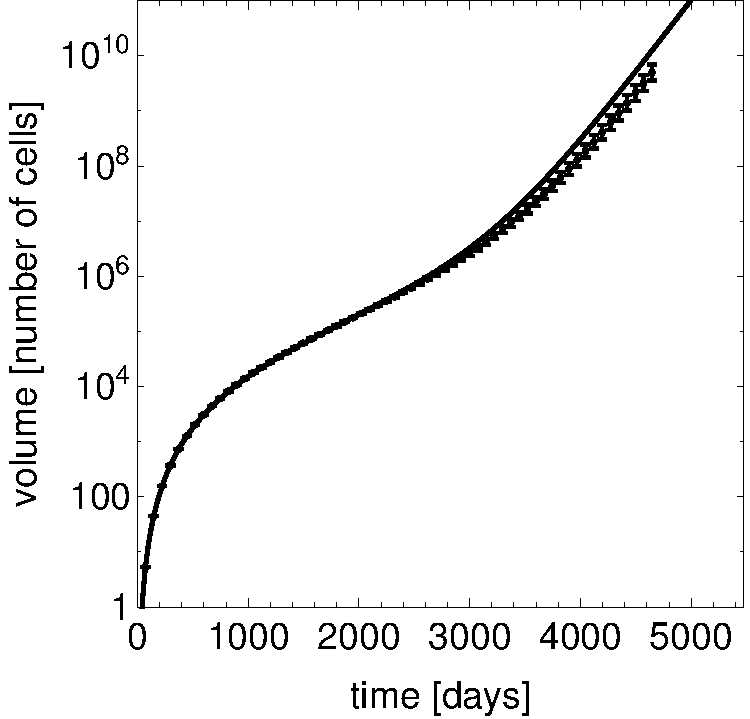
\includegraphics[width=1\textwidth]{images/SimpleModel3.pdf} 
        \column{0.5\textwidth}
        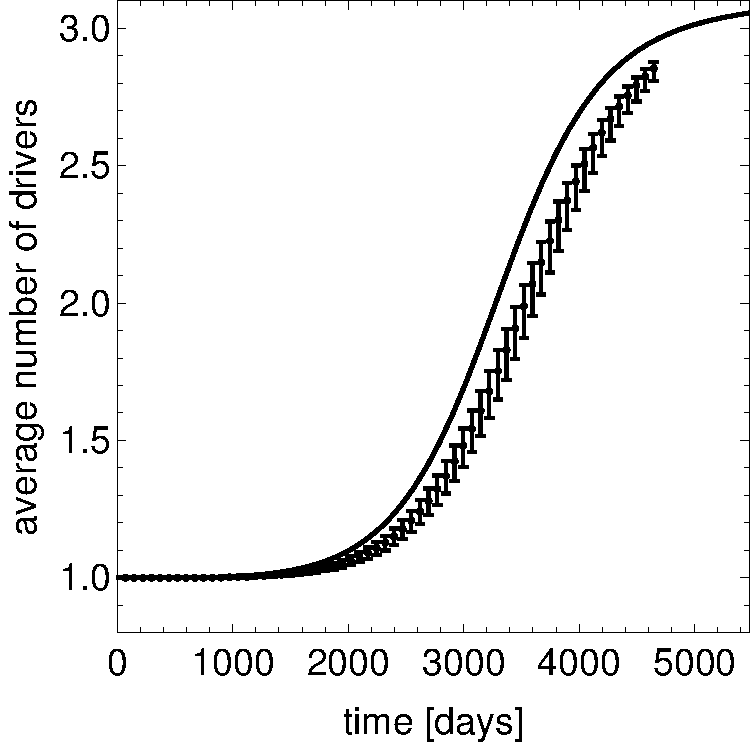
\includegraphics[width=1\textwidth]{images/SimpleModel4.pdf} 
    \end{columns}
\end{frame}

\begin{frame}
\frametitle{How could invasion affect evolution?}
\begin{columns}[c]
    \column{0.5\textwidth}
    \colorbox{white}{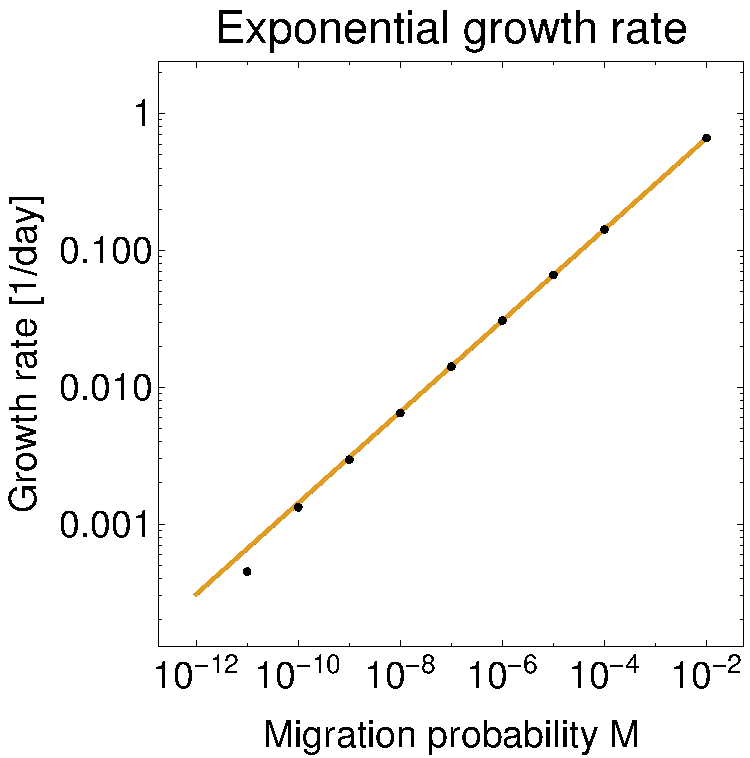
\includegraphics[width=1\textwidth]{images/SimpleGR.pdf} }
    \column{0.5\textwidth}
    \begin{itemize}
        \item Growth \emph{exponential}
        \item Consistent with clinical doubling times
        \item PREDICTION: higher motility $\rightarrow$ higher \emph{fitness}
    \end{itemize}
\end{columns}
\end{frame}

\begin{frame}
    \frametitle{What about branching/complex pathways?}

    \begin{center}
    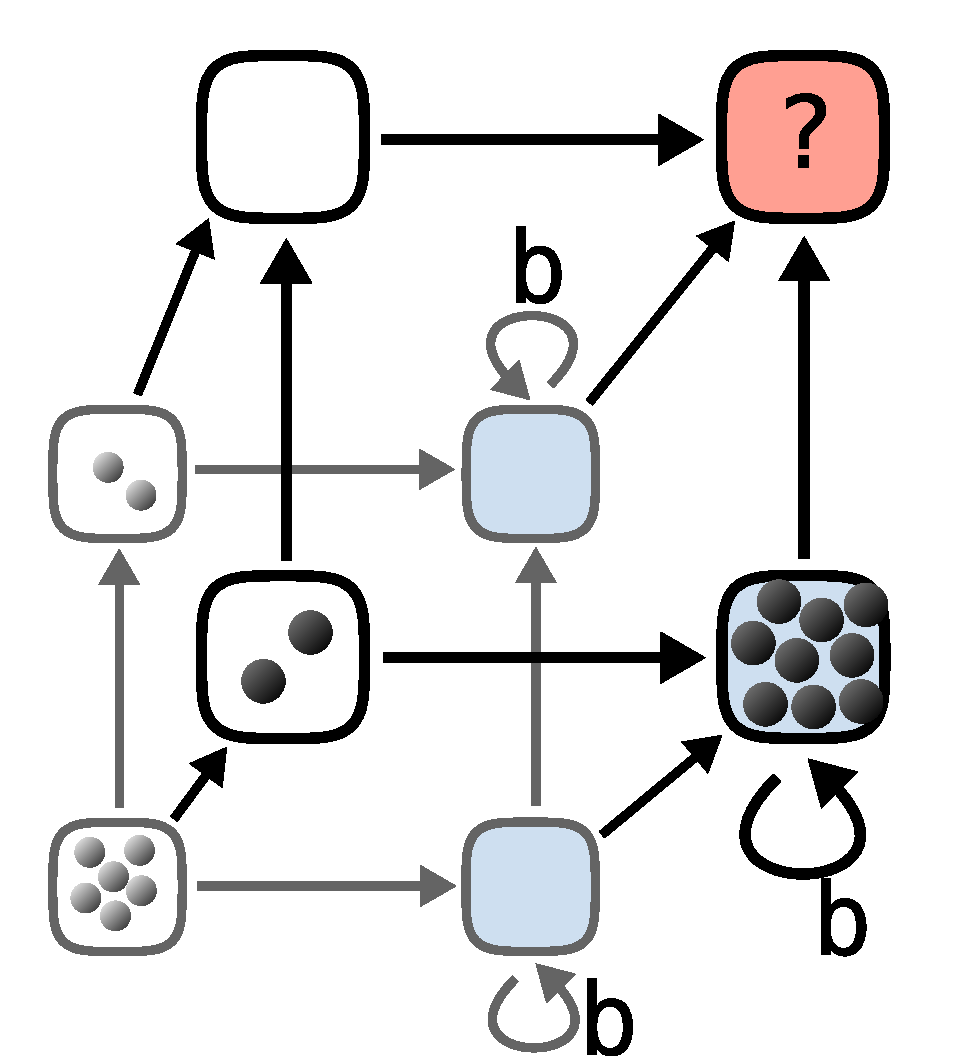
\includegraphics[width=0.65\textwidth]{images/cubegraph.pdf}
    \end{center}
\end{frame}

\begin{frame}
    \frametitle{Colorectal adenocarcinoma}
    % Diagram of three different genes being mutated: two lost, one activated

    \begin{center}
    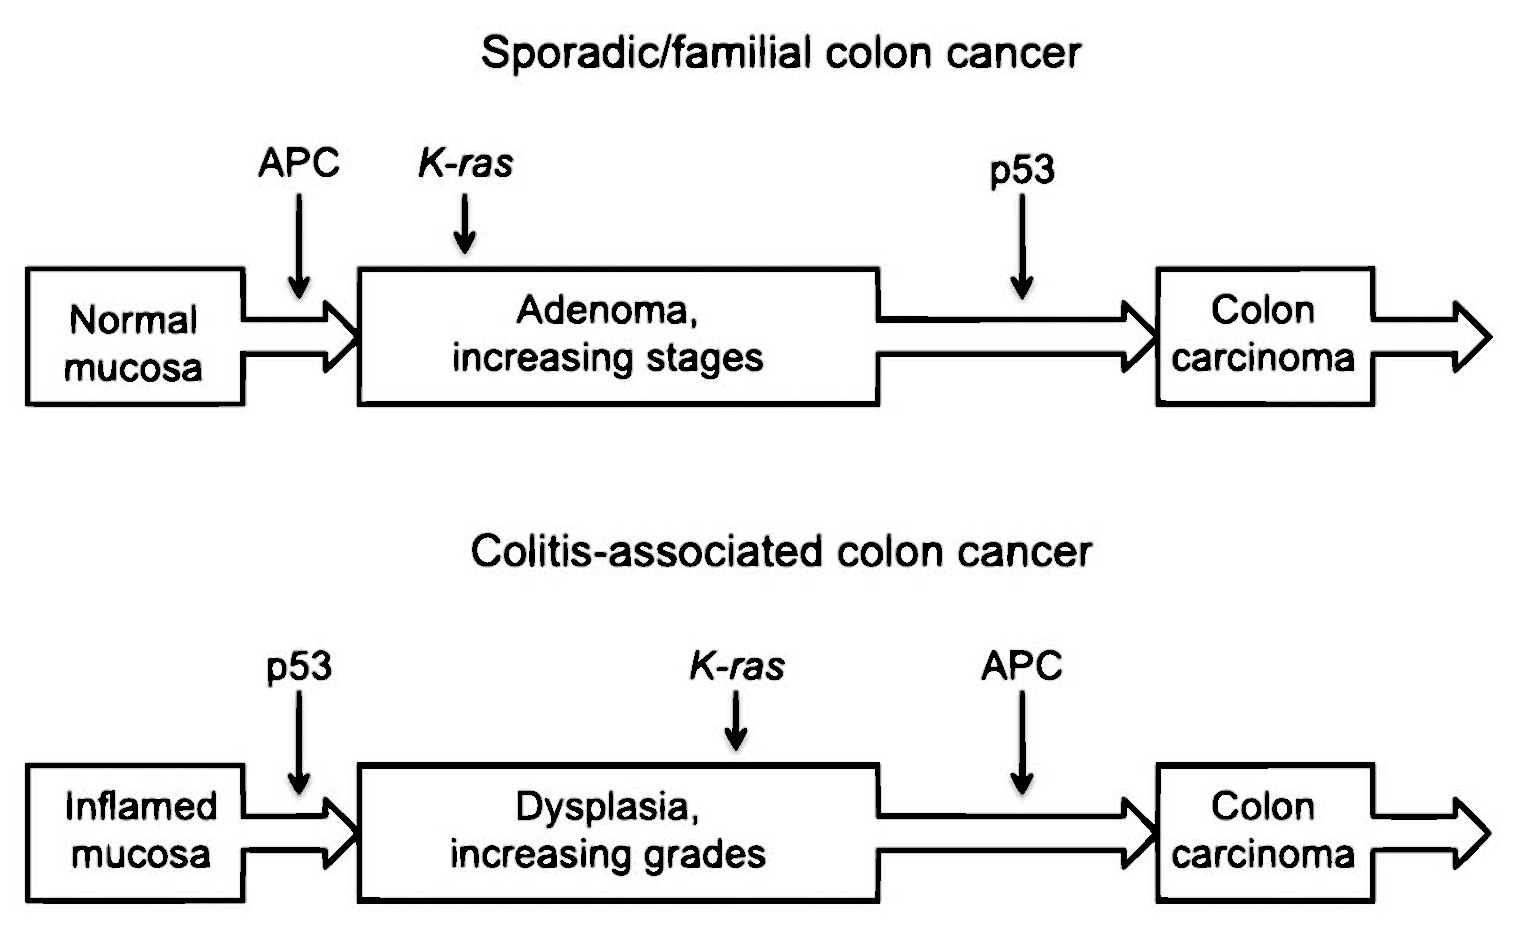
\includegraphics[width=1.0\textwidth]{images/IJO-45-03-0959-g00.pdf}
    \end{center}

    \tiny{A. De Lerma Barbaro \emph{et al.}, ``Inflammatory cues acting on the adult
    intestinal stem cells and the early onset of cancer'', International
    Journal of Oncology, 45(3) 2014.}
\end{frame}

\begin{frame}
    \frametitle{Colorectal adenocarcinoma}

    \begin{center}
    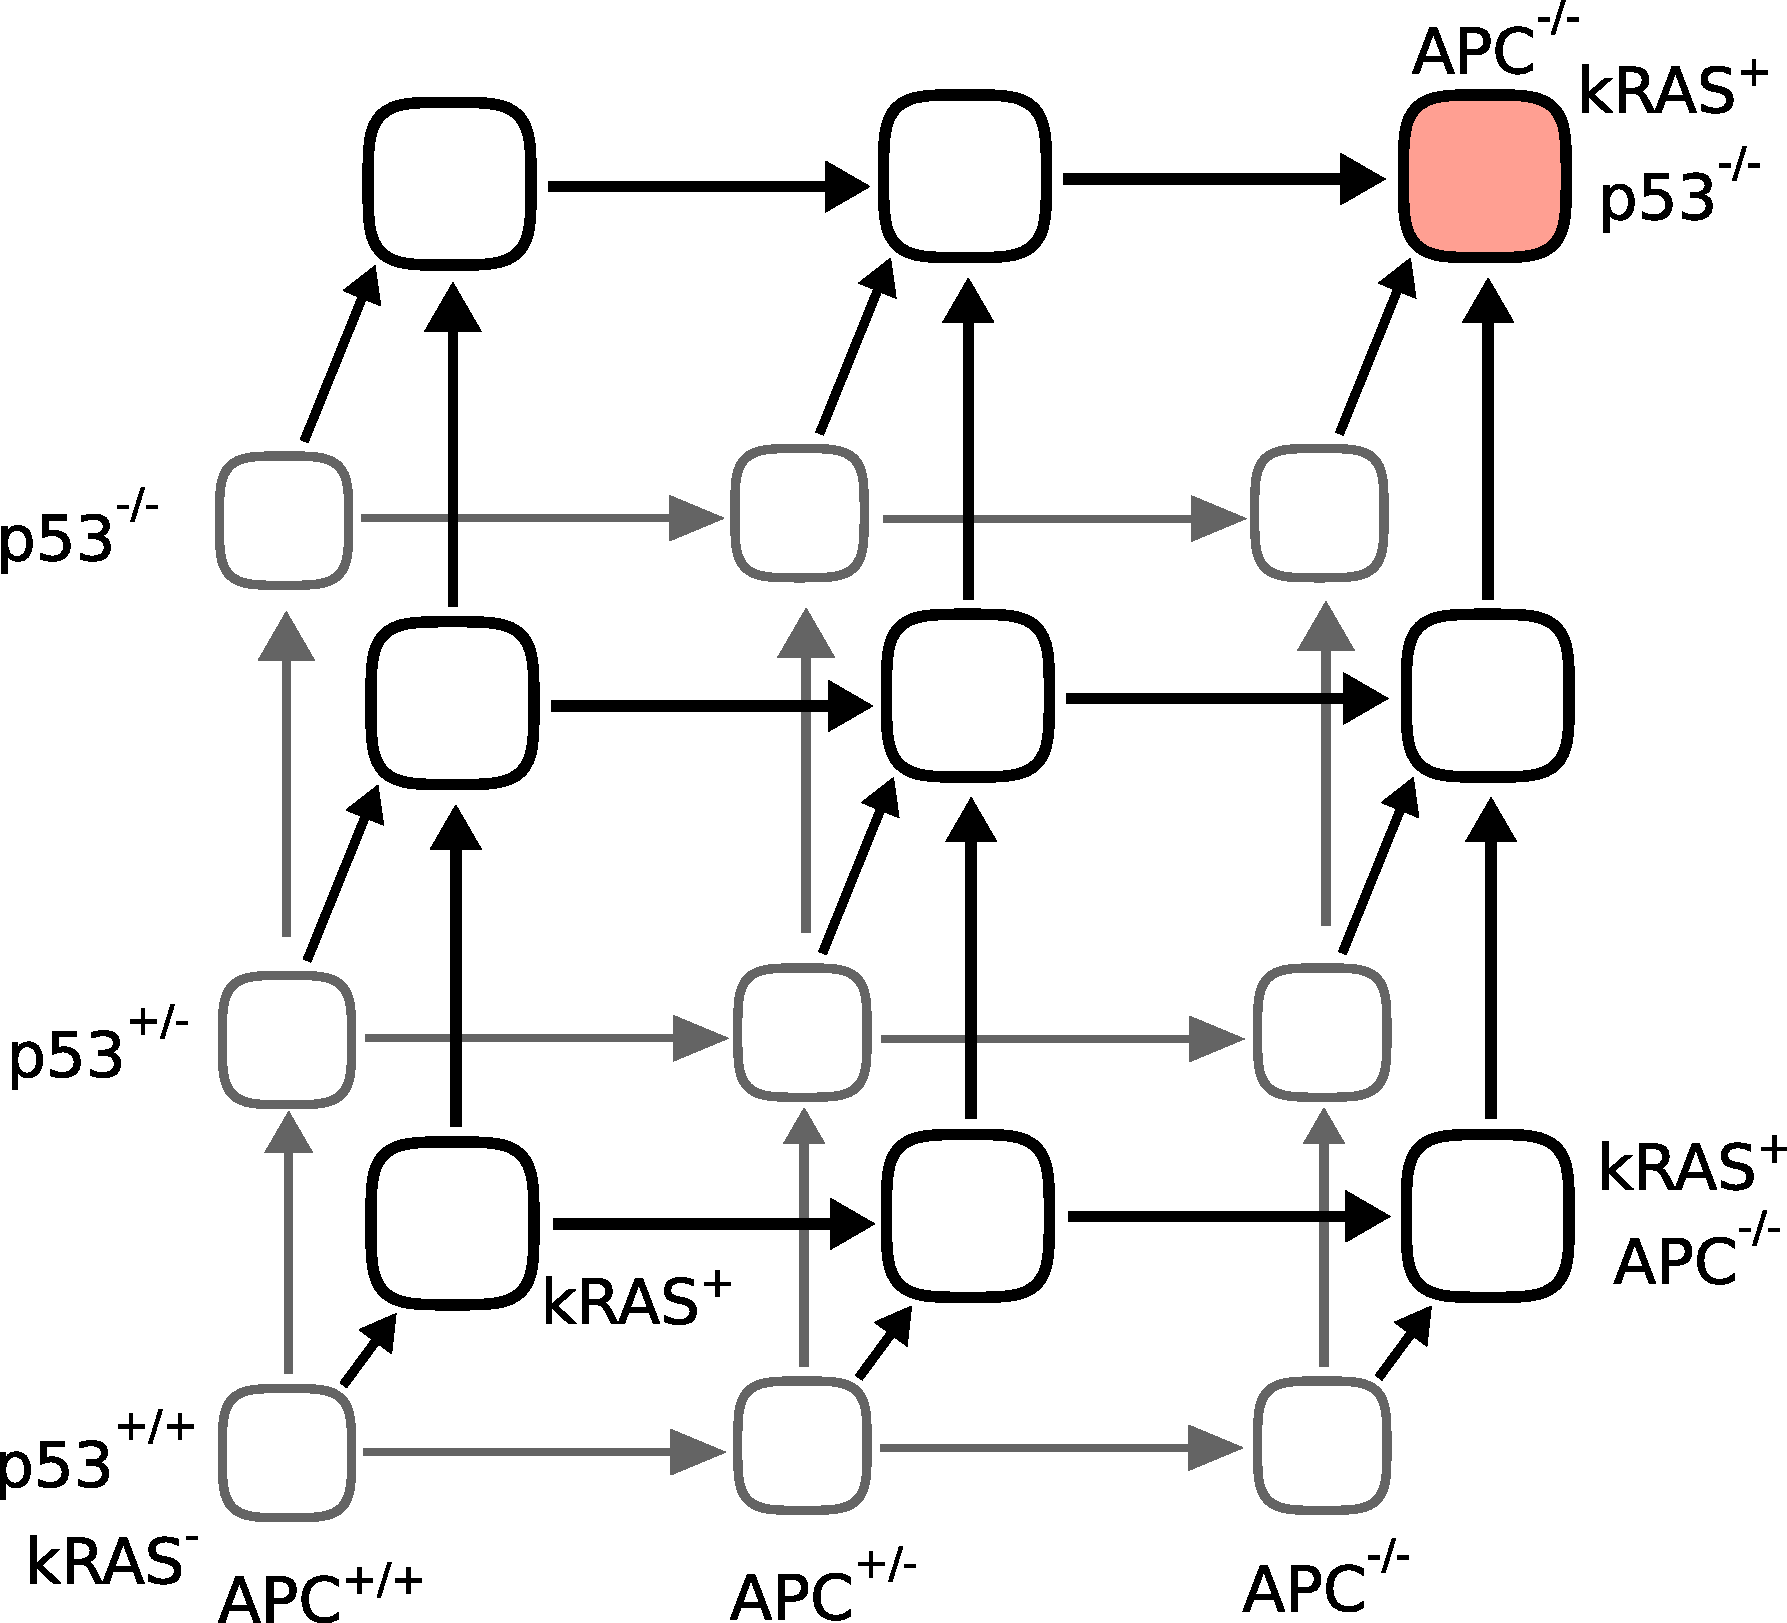
\includegraphics[width=0.8\textwidth]{images/cubegraph2.pdf}
    \end{center}

\end{frame}

\begin{frame}
    \frametitle{Colorectal adenocarcinoma}

    \begin{center}
    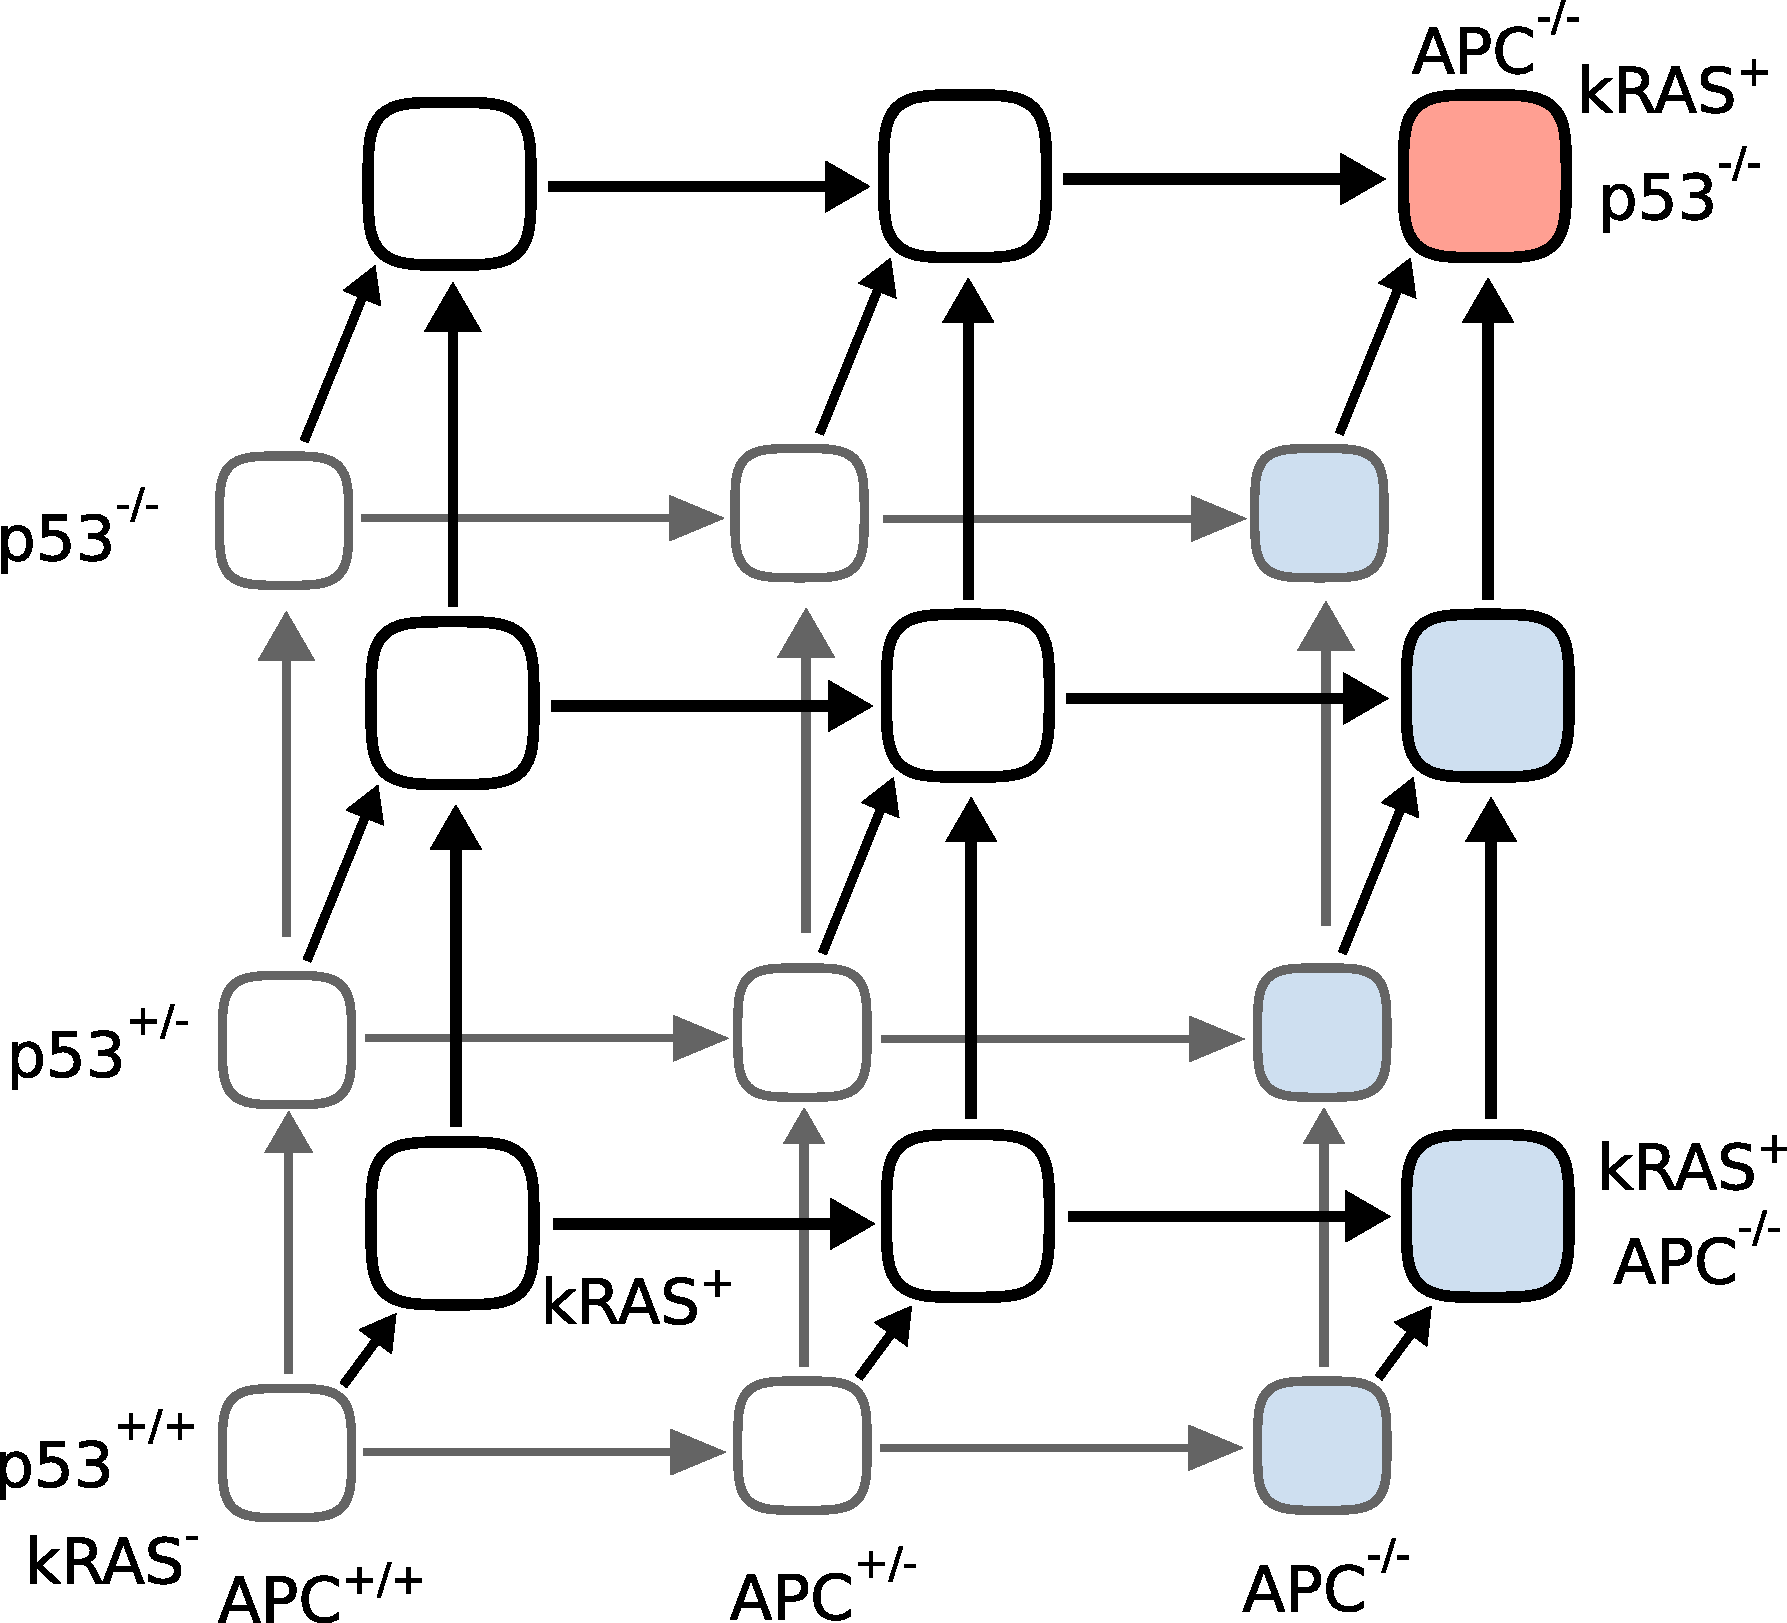
\includegraphics[width=0.8\textwidth]{images/cubegraph3.pdf}
    \end{center}

\end{frame}

\begin{frame}
    \frametitle{Colorectal adenocarcinoma}

    \begin{center}
    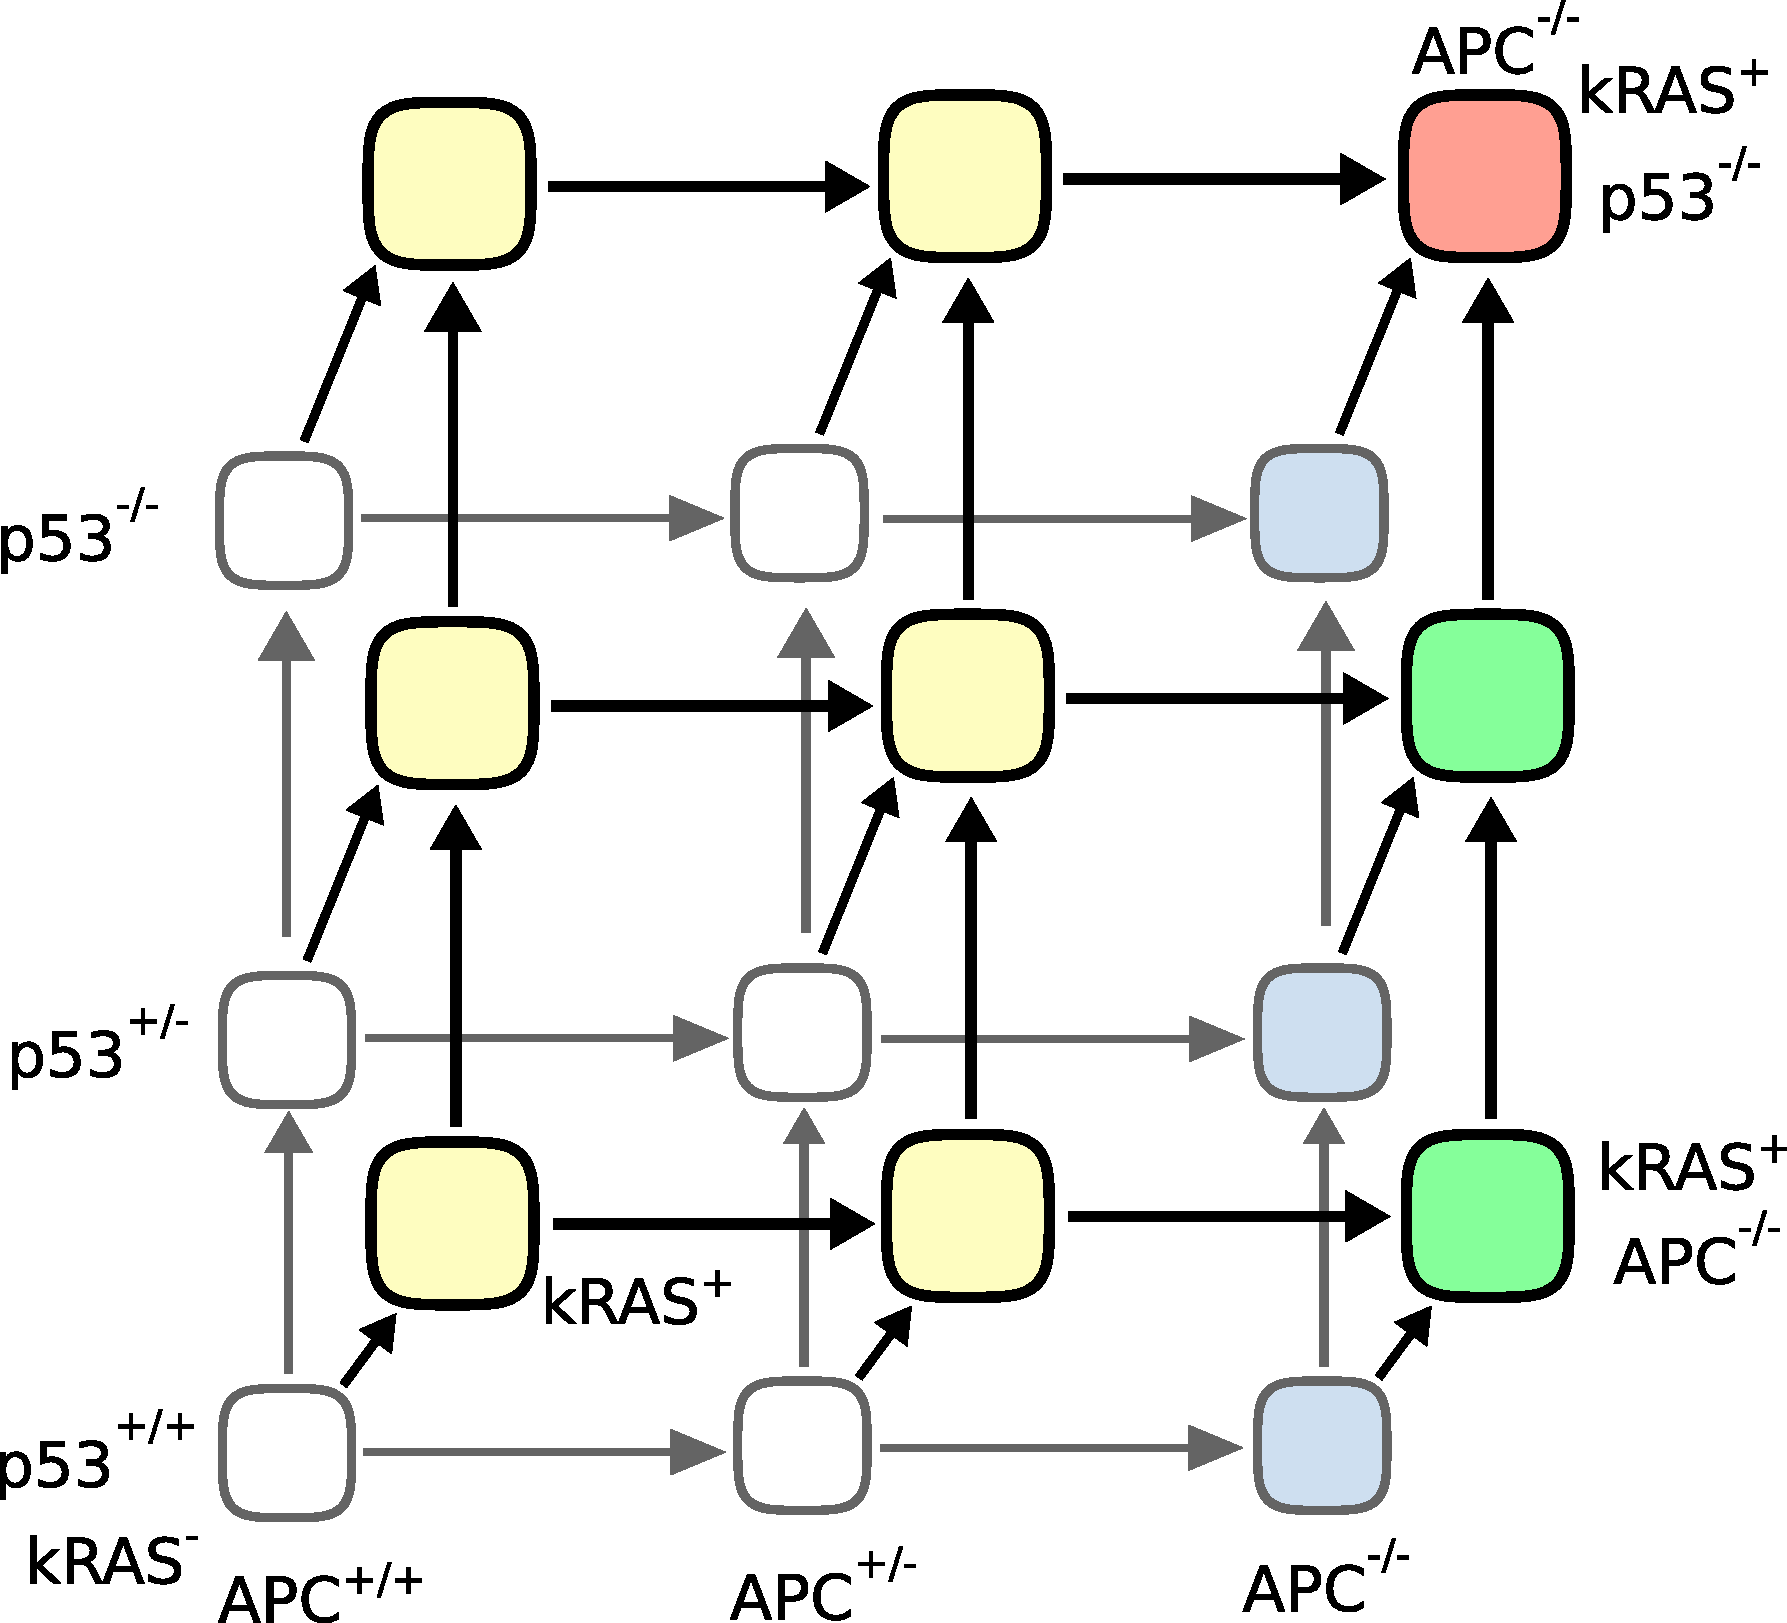
\includegraphics[width=0.8\textwidth]{images/cubegraph4.pdf}
    \end{center}

\end{frame}

% 5 mutations necessary
% 5! = 120 possible orders
% (some of these are not biologically possible)
% Does the order matter?

\begin{frame}
    \frametitle{The speed of cancer evolution}
    In the limit that mutation is rare compared to growth, these are:

    \begin{align}
        Pr(\mathrm{cancer}) &\approx \frac{1}{4} N r_{APC} r_{tp53} r_{kRAS} r_{LOH}^2 \cdot t^5 \\
        Pr(\mathrm{cancer}) &\approx \frac{3}{2} N \frac{r_{APC} r_{tp53} r_{kRAS} r_{LOH}^2}{b_1^3}
        \cdot t^2 e^{b_1 t} \\
        Pr(\mathrm{cancer}) &\approx c N r_{APC} r_{tp53} r_{kRAS} r_{LOH}^2 \tau^4 \cdot t\; e^{b_{12} t}
    \end{align}

    (compare Armitage \& Doll 1954), where

    \begin{equation*}
        \tau^4 = \frac{1}{b_{12}^3 (b_{12}-b_1)} + \frac{1}{b_{12}^3 (b_{12}-b_2)} +
            \frac{1}{b_{12}^2 (b_{12}-b_2)^2}
    \end{equation*}

    \;
    \hrule
    \;

    \tiny{Ivana Bozic\*, Chay Paterson, Hans Clevers, ``Mathematical model of
    colorectal cancer initiation'', (pending submission), 2019}
\end{frame}

\begin{frame}
    \frametitle{How does evolution affect lifetime risk?}

    \begin{center}
    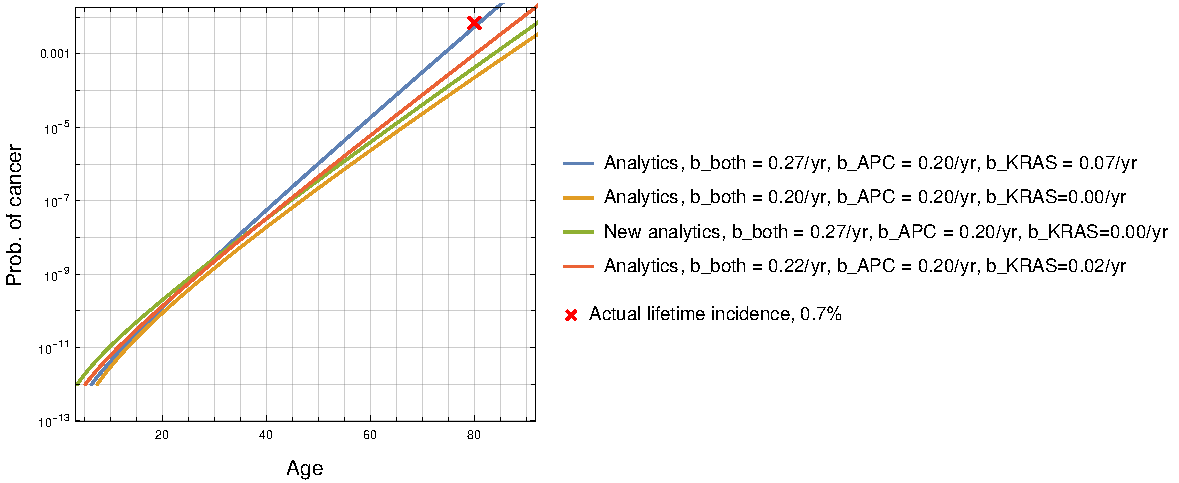
\includegraphics[width=1.0\textwidth]{images/LastPlot.pdf}
    \end{center}

    \;
    \hrule
    \;

    \tiny{Ivana Bozic\*, Chay Paterson, Hans Clevers, ``Mathematical model of
    colorectal cancer initiation'', (pending submission), 2019}

    \tiny{(2) C. Tomasetti, B. Vogelstein, ``Variation in cancer risk among
    tissues can be explained by the number of stem cell divisions'',
    \emph{Science} 347(78-81) (2015).}
\end{frame}

\begin{frame}
\frametitle{Conclusions}
    \begin{itemize}
        \item Motility can ``boost'' fitness.
        \item Fitness differentials accelerate cancer evolution.
        \item Current experimental knowledge \emph{can} explain incidence.
        \item All of our inputs are empirically measurable. 
        \item The main output, incidence against age, is also measurable.
    \end{itemize}
\end{frame}

\begin{frame}
    \frametitle{Open questions}
    Application to other cancers/disorders?
    \begin{itemize}
        \item Familial adenomatous polyposis?
        \item Bloom syndrome?
    \end{itemize}

    ``Inverse problem'': can different molecular subtypes be deduced from
    incidence data?
\end{frame}
\end{document} 
